\documentclass[11pt,letterpaper]{article}
\usepackage[latin1]{inputenc}
\usepackage{amsmath}
\usepackage{amsfonts}
\usepackage{amssymb}
\usepackage{graphicx}
\usepackage{capt-of}

\setlength{\parskip}{1pc}
\setlength{\parindent}{0pt}
\setlength{\topmargin}{-3pc}
\setlength{\textheight}{9.0in}
\setlength{\oddsidemargin}{0pc}
\setlength{\evensidemargin}{0pc}
\setlength{\textwidth}{6.5in}

\title{6.170 Assignment 1 Documentation}
\author{Dina Betser}


\begin{document}
\maketitle

\section{Models}
\subsection{Object Models}
The object model for the problem domain is included in the figure below. The problem domain object model demonstrates the system that must be built. A photo \texttt{Gallery} corresponding to a \texttt{Directory} of \texttt{Photo}s. Each \texttt{Photo} in the directory is preceded by the previous \texttt{Photo} in the \texttt{Directory} and followed by the next \texttt{Photo}. Every \texttt{Photo} has a \texttt{Caption} made up of metadata fields from the set of \texttt{IPTC Info Elements}\footnote{The IPTC Info elements include: date created, digital creation date, reference number, custom8, custom9, sub-location, object cycle, custom4, custom5, custom6, custom7, custom1, custom2, reference date, by-line title, local caption, keywords, province/state, category, custom17, custom14, digital creation time, custom12, custom13, custom10, custom11, headline, custom18, custom19, source, contact, by-line, object name, content location code, language identifier, release date, expiration date, reference service, custom16, original transmission reference, originating program, subject reference, city, supplemental category, content location name, country/primary location code, editorial update, custom15, fixture identifier, custom3, country/primary location name, action advised, custom20, copyright notice, program version, image orientation, edit status, expiration time, release time, credit, time created, special instructions, writer/editor, caption/abstract, urgency, and image type.}.
\begin{center}
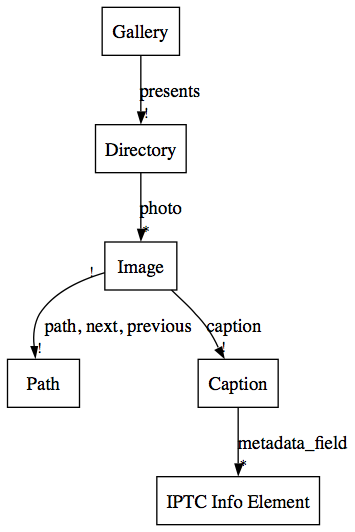
\includegraphics[width=200pt]{dot/obmod.png}
\label{fig:ob1} 
\end{center}

I was not sure what the abstract state object module should look like, as the final application is composed of static HTML, which does not store state.

\section{Design Notes}
\subsection{Key Challenges}
\begin{itemize}
\item Getting acquainted with Jinja and valid HTML best practices. 
\item Organizing the code to encapsulate the interaction with the file system, the Jinja templates, and the image data.
\item Using just HTML/CSS to show one image at a time. Reused a CSS code snippet for this.
\item Representing an image with all of its necessary components.
\end{itemize}

\subsection{Issues Arising}
\begin{itemize}
\item Images that did not have values for the desired metadata fields.\\
For images without values for desired metadata fields, I simply returned a default message stating that the field was empty.
\item HTML did not validate using the validator.\\
Previously, I was using the doctype declaration of \texttt{<!DOCTYPE html>}. I switched the doctype to \texttt{<!DOCTYPE html PUBLIC "-//W3C//DTD HTML 4.01 Transitional//EN">} to resolve the validation issues. I also needed to do things like ensure that the title of any image did not start with a number, so I prepended the word ``photo'' to ensure that all titles started with a valid character.
\item Storing a pointer to the previous and next photo in the directory.\\
In the first version of my implementation, I did not facilitate ImageDataObjects being aware of the predecessors and successors within the directory. I added a \texttt{prev} and \texttt{next} field in the \texttt{ImageDataObject} class to solve this issue.
\end{itemize}

\subsection{Critique}
This project required a clear understanding of each Python class that was used. Each class I created had a clear specification and purpose, so the code itself was organized fairly well.

The \texttt{ImageDataObject} data structure was particularly succinct at storing all of the information required to display a photo in the gallery.

The implementation was the most basic of the possible implementations that fulfilled the requirements. No nested directories were supported and options to the Python script needed to be provided as command line arguments, not by the user viewing the application, which is less user-friendly.
\section{Specification}
\subsection{Overview}
This application generates a static HTML website that works as a browser-based photo gallery implementation. The gallery allows users to view photos stored locally to the directory where the script is run. Users may specify which metadata fields they wish to use as captions in the gallery. They may scan through the collection of images by clicking the left and right arrow buttons. All effects are achieved without the use of Jacascript; only HTML and CSS along with the Python Jinja2 library are used for this project.
\subsection{Key Features}
The key features of this implementation of the 6.170 photo gallery are:
\begin{itemize}
\item Minimalist, intuitive interface for scanning through photos in the gallery.
\item Images are displayed in the center of the UI, attracting attention. The caption is displayed below the photo, where users would expect it.
\item Generated HTML depends on multiple command-line arguments that can customize the files used and the output of the script.
\end{itemize}
\subsection{User Manual}
To run the code, python2.6 must be installed, with the jinja2 module and the iptcinfo module available.

The 6.170 photo gallery is a static HTML page that is generated via a Python script that uses the Jinja templating system. The HTML is generated by running a python script with command-line arguments specifying options.
For example, a sample run of the script to generate the html file photo\_gallery.html might look like:
\begin{verbatim}
$ python2.6 photo_gallery.py images/ photo_gallery.html caption/abstract
templates/photo_gallery_template.html
\end{verbatim}
In this case, the arguments are as follows:
\begin{verbatim}
$ python2.6 photo_gallery.py <image_directory> <output_filename> <comma-separated list of
metadata fields> <input_filename>
\end{verbatim}

The user may only specify a single directory from which to generate the gallery, and no subdirectories are included in the gallery. This image directory must be specified with a slash (\/) following the name.


\section{Implementation}

\subsection{Module Dependency Diagram}
This code's modules can only be seen as the member variables of classes, since there was only one Python module involved in the code generation.
\begin{center}
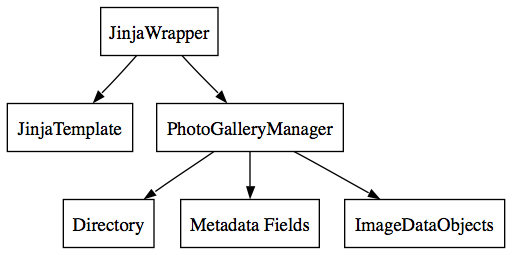
\includegraphics[width=250pt]{dot/moddepdiagram.png}
\label{fig:ob2} 
\end{center}
\subsection{Code Notes}
This code was fairly straightforward to write. The biggest issue I had was determining how to display only one photo, with previous and next buttons, using only HTML and CSS.

\section{Testing}

\subsection{Test Plan}
To test the application, the generated HTML was inspected in multiple browsers, including Safari, Chrome, and Firefox.

The testing for this project was mostly manual since it was a more contained project.
\subsection{Test Cases}
Tested the code on the sample photos, which displayed properly.

It was determined that the buttons scan through the photos as desired.

The captions are displayed even when multiple IPTCInfo elements are included. This was tested by including the caption/abstract element twice, which worked properly by including the photo abstract twice in the caption on the website.

The HTML was validated to ensure standards compliance.
\begin{verbatim}
$ python2.6 photo_gallery.py images/ photo_gallery.html caption/abstract,caption/abstract 
templates/photo_gallery_template.html
\end{verbatim}

\subsection{Rationale and Conclusions}
This code fulfills the requirements of the assignment, but doesn't go much beyond that. The product, when run with expected and well-formed inputs, runs exactly as desired. It may fail in unexpected ways with malformed input.
\end{document}

